\message{ !name(recursion.tex)}\documentclass[fleqn, t]{beamer}

\usetheme[block=fill,numbering=none,sectionpage=none,subsectionpage=progressbar]{metropolis}

\title{Recursion}
\subtitle{Module 12}
\author{Tushaar Kamat}
\date{\today}

\begin{document}

\message{ !name(recursion.tex) !offset(-3) }


\maketitle

\begin{frame}
  \frametitle{Outline}
  \tableofcontents
\end{frame}

\section{Recursion Concepts}
\subsection{Introduction}
\begin{frame}
  \frametitle{What is Recursion?}
  \begin{itemize}[<+->]
  \item The easiest definition of recursion is a task that gets repeated
    infinitely until a base case is reached, at which it ``steps'' back to its
    origin. 
  \item Often, recursive programs look deceivingly short compared to their
    iterative counterparts, but they get the job done just as well.
  \item Once you step into the land of the recursion, there is no going back!
  \end{itemize}
  \begin{figure}
    \onslide<4->{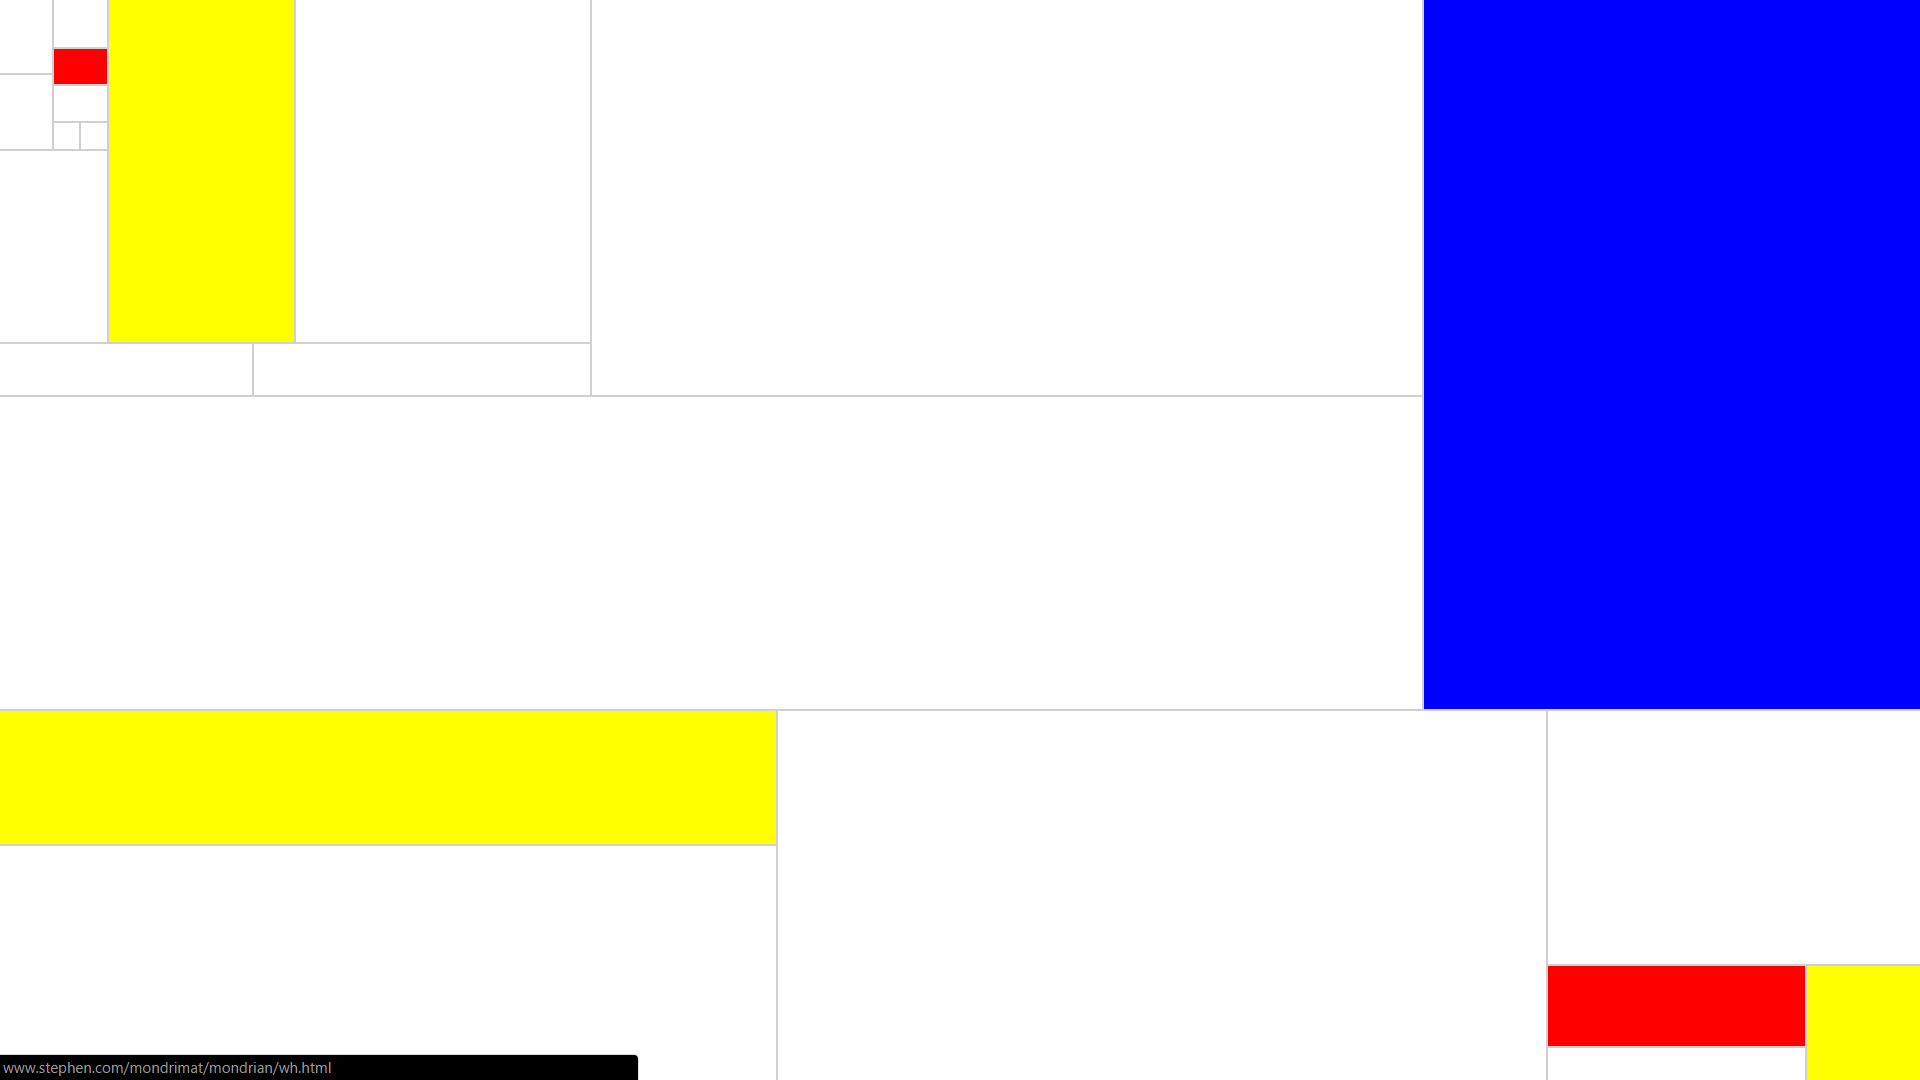
\includegraphics[scale=0.10]{Mondrian.png}
      {\caption{My Attempt at Recursive Mondrian Art}}}
  \end{figure}

\end{frame}
\begin{frame}
  \frametitle{Recursion Analogies}
  \begin{itemize}[<+->]
  \item Whether through Russian dolls or through factorials and Fibonacci
    numbers, everyone has a different way of understanding recursion. 
  \item My first introduction to recursion was with two opposite mirrors in my
    bathroom, it was always interesting to see how they went on and on forever!
  \end{itemize}
  \begin{figure}
    \onslide<3->{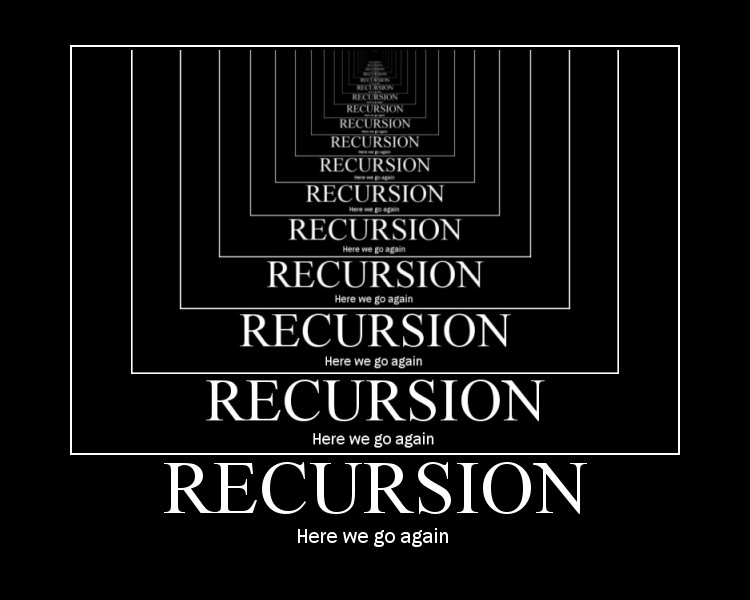
\includegraphics[scale=0.15]{mirrors.png}}
  \end{figure}
\end{frame}

\subsection{Divide and Conquer}
\begin{frame}[c]
  \frametitle{Divide and Conquer}
  \begin{columns}[t]
    \begin{column}{.4\textwidth}
      \begin{block}{Steps for Recursive Problem}
        \begin{enumerate}[<+->]
        \item Identify the base case.
        \item Determine the recursive call.
        \item Break the program down into small pieces to form a whole.
        \end{enumerate}
      \end{block}
    \end{column}

    \begin{column}{.6\textwidth}
      \begin{figure}
        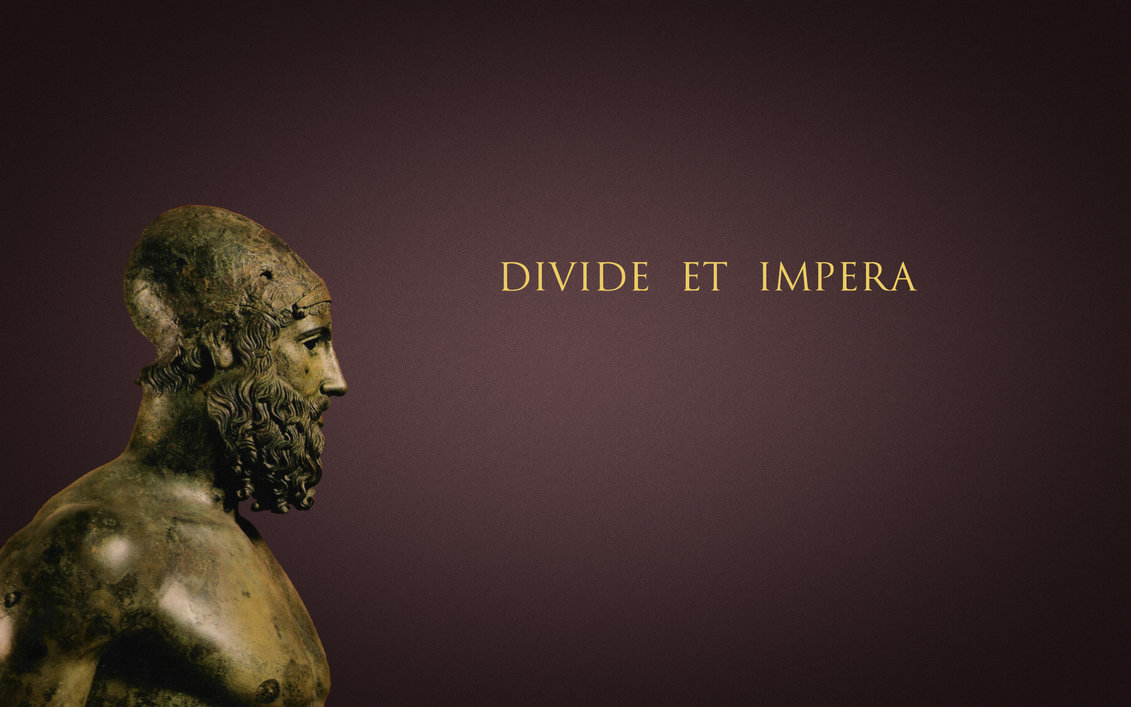
\includegraphics[scale=0.2]{divide.jpg}
      \end{figure}

    \end{column}
  \end{columns}

\end{frame}
\begin{frame}
  \frametitle{Recursive Factorials}
  \begin{itemize}[<+->]
  \item Factorials are a great way to understand divide and conquer.  
  \item Since $n!$ can be defined as $n \cdot (n-1)!$, and $0!$ = 1, factorial
    problems can easily be solved with recursion. 
  \end{itemize}
  \begin{block}{Steps for Recursive Factorial}
    \begin{enumerate}[<+->]
    \item $5!$
    \item $5 \cdot 4!$
    \item $5 \cdot 4 \cdot 3!$ 
    \item $5 \cdot 4 \cdot 3 \cdot 2!$
    \item $5 \cdot 4 \cdot 3 \cdot 2 \cdot 1!$
    \item $5 \cdot 4 \cdot 3 \cdot 2 \cdot 1 \cdot 0!$ ($0!$ is $1$)
    \item $= 120$
    \end{enumerate}
  \end{block}
\end{frame}

\section{Piecewise Functions}
\subsection{Introduction}
\begin{frame}
  \frametitle{What are Piecewise Functions?}
  \begin{itemize}[<+->]
  \item Piecewise functions are basically functions that take paths based on
    conditions, often calling themselves with a different value. 
  \item For a piecewise function to not be infinite, it must have a ``base case'',
    and the other cases must approach it.
  \end{itemize}
  \onslide<3->{
    \begin{example}
      \begin{equation*}
        f(x)= 
        \begin{cases}
          f(x - 1) + 2 & \text{if } x > 10 \\
          8 & \text{if } x \leq 10
        \end{cases}
      \end{equation*}
    \end{example}
  }
\end{frame}

\begin{frame}
  \frametitle{Solving Piecewise Functions}
  \begin{itemize}[<+->]
  \item Solving piecewise functions involves a simple strategy called
    Simplify-Substitute-Solve, or S-S-S. 
  \end{itemize}
  \begin{block}{S-S-S Strategy}
    \begin{enumerate}[<+->]
    \item Simplify - Plug and chug until you reach the base case. 
    \item Substitute - Use the base case in the last unsolved expression. 
    \item Solve - Work your way back up to the top of the expression.
    \end{enumerate}
  \end{block}
  \begin{figure}
    \onslide<5->{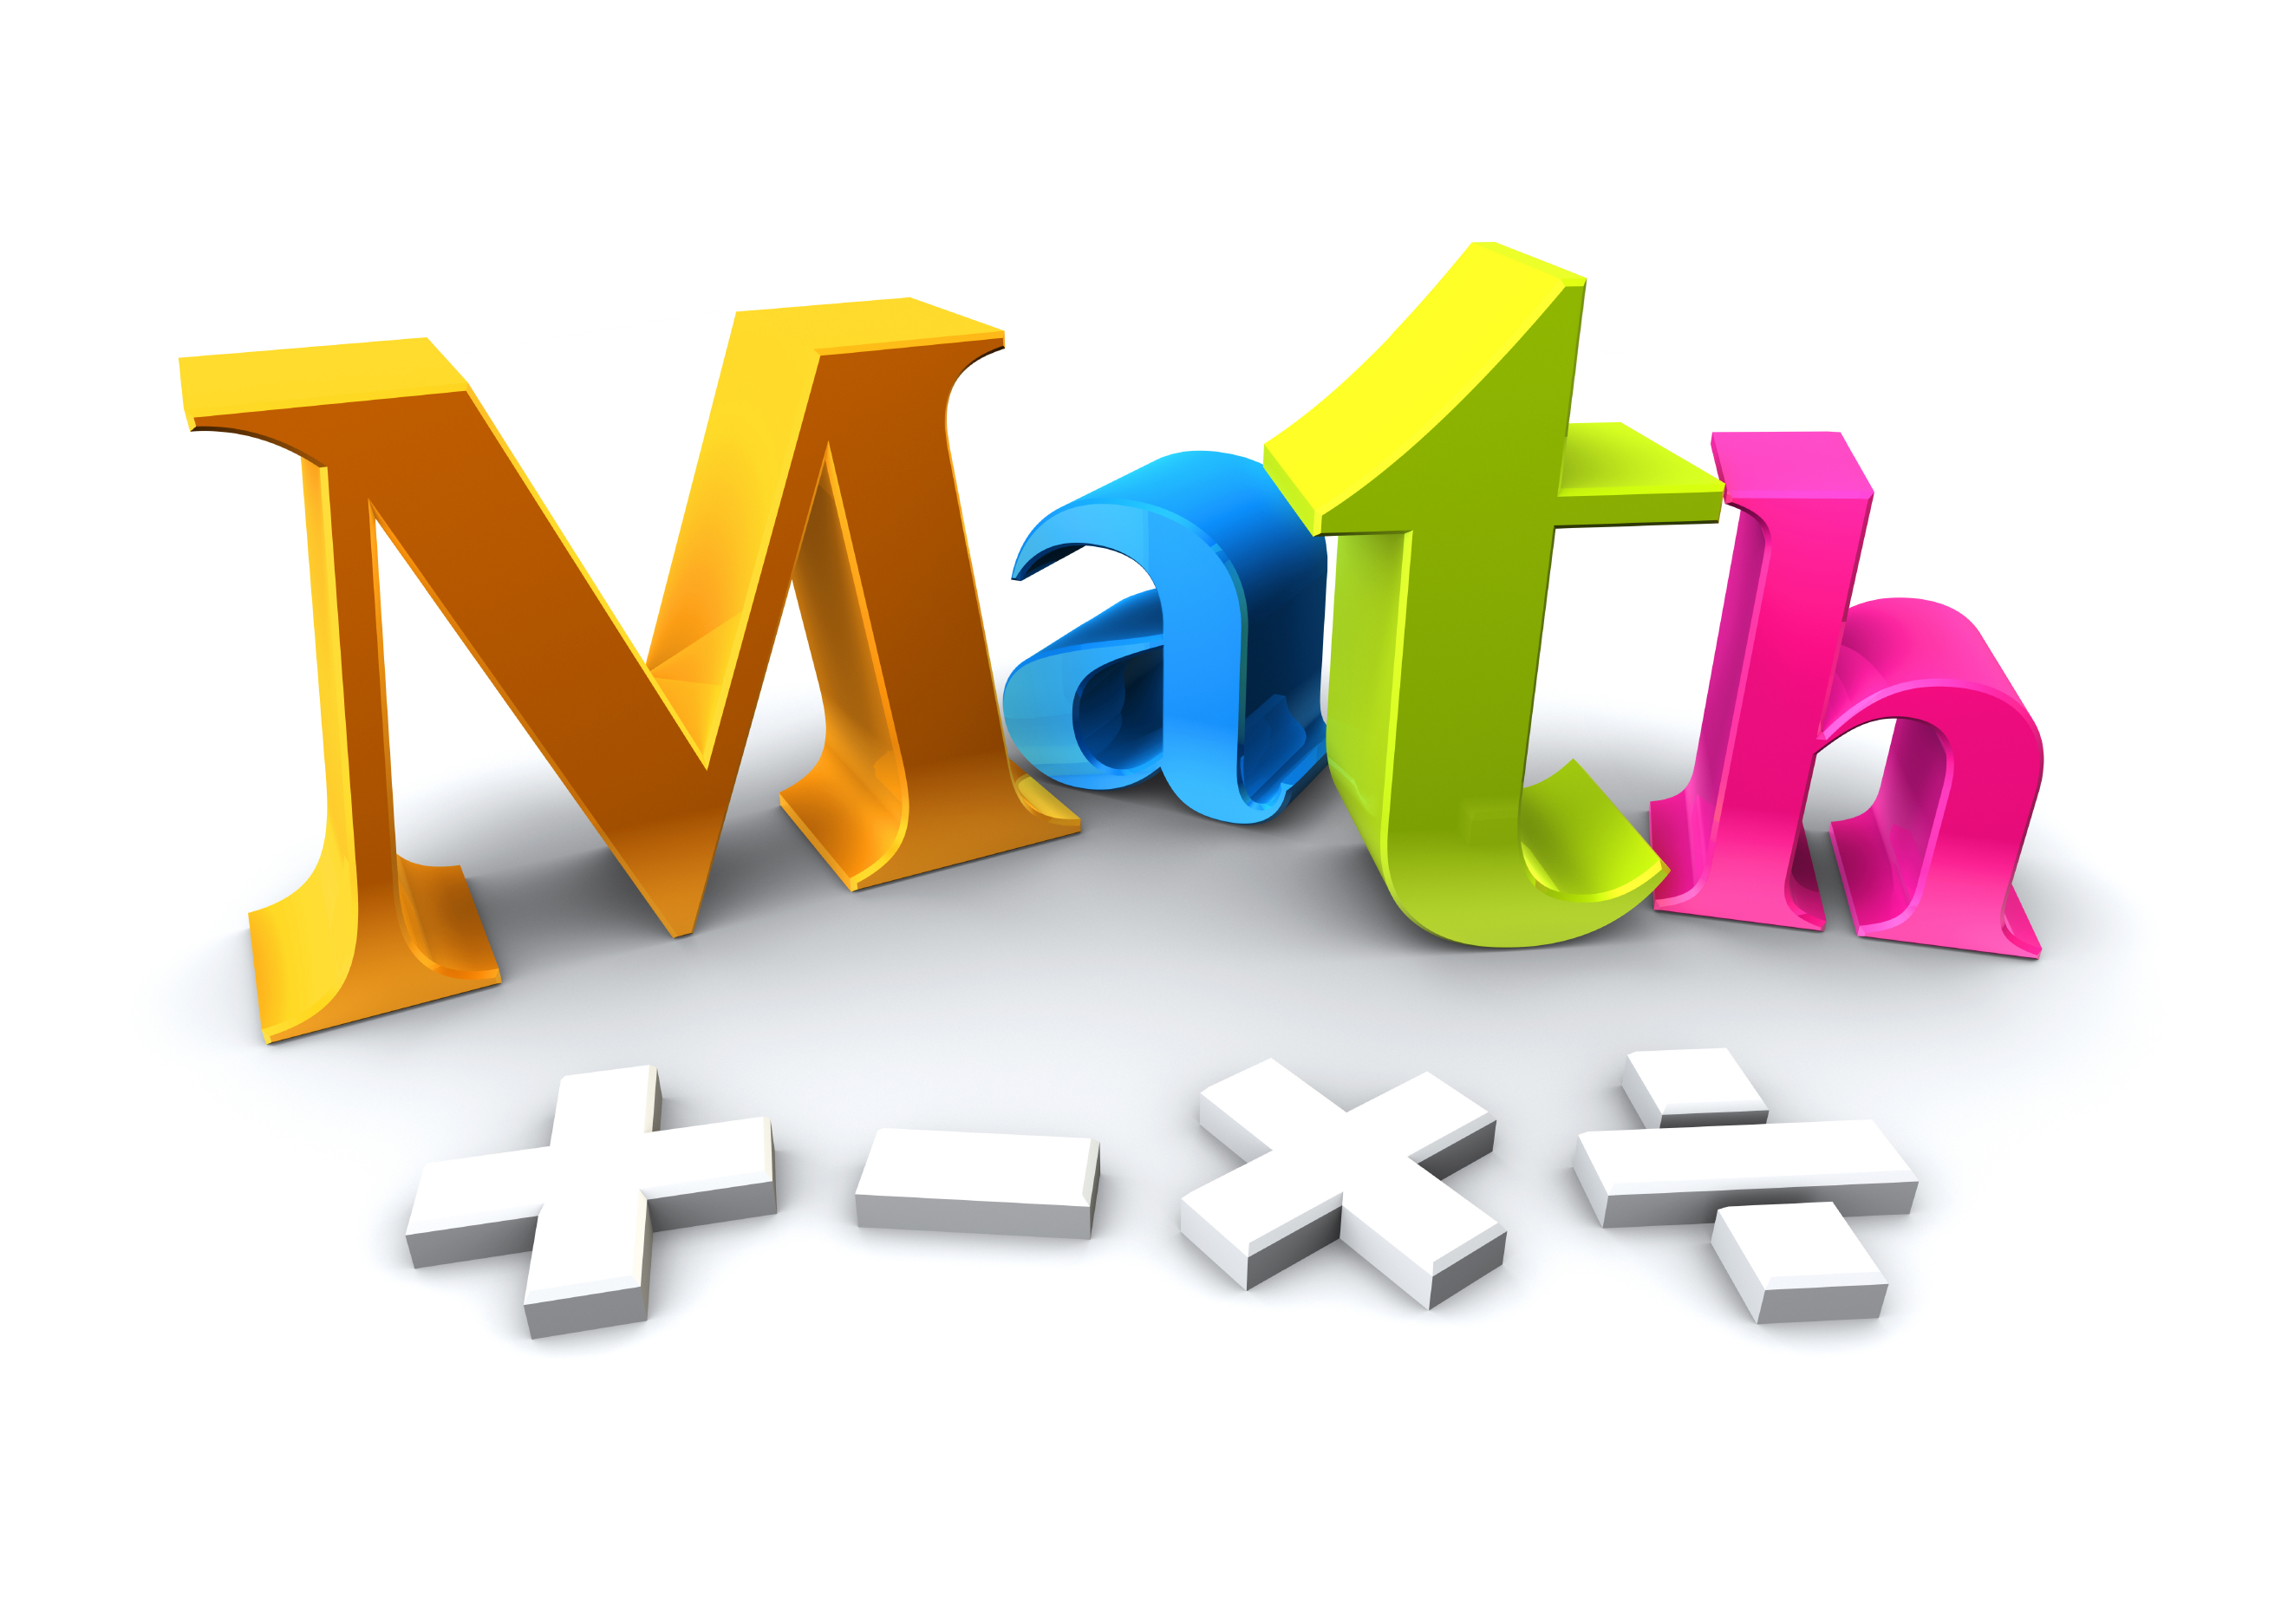
\includegraphics[scale=.06]{math.jpg}}
  \end{figure}
\end{frame}

\subsection{Examples}

\begin{frame}
  \frametitle{Factorials Revisited}
  \begin{block}{Factorial Piecewise Function}
    \begin{equation*}
      f(x) = 
      \begin{cases}
        f(x - 1) \cdot x & \text{if } x > 0\\
        1 & \text{if } x = 0
      \end{cases}
    \end{equation*}
  \end{block}
  \begin{itemize}[<+->]
  \item This piecewise equation should seem very familiar; it uses the exact
    same concept as the recursive factorial shown earlier!
  \end{itemize}
  \begin{figure}
    \onslide<2->{
\includegraphics[scale=0.25]{mind}}
  \end{figure}
\end{frame}

\begin{frame}
  \frametitle{Working Through a Piecewise Function}
  \begin{block}{Piecewise Function}
    \begin{equation*}
      f(x)= 
      \begin{cases}
        f(x - 1) + 2 & \text{if } x > 10 \\
        8 & \text{if } x \leq 10
      \end{cases}
    \end{equation*}
  \end{block}
  \begin{itemize}[<+->]
  \item Here is the example from a few slides ago. 
  \item If you wanted to solve for $x = 14$, you could do as follows \dots
  \end{itemize}
  \begin{block}{Simplify}
    \begin{enumerate}[<+->]
    \item $f(14) : 14 > 10 : f(14 - 1) + 2$
    \item $f(13) : 13 > 10 : f(13 - 1) + 2$
    \item $f(12) : 12 > 10 : f(12 - 1) + 2$
    \end{enumerate}
  \end{block}
\end{frame}

\begin{frame}
  \frametitle{Working through a Piecewise Function (Continued)}
  \begin{block}{Simplify}
  \begin{enumerate}[<+->]
    \setcounter{enumi}{3}
  \item $f(11) : 11 > 10 : f(11 - 1) + 2$
  \item $f(10) : 10 \leq 10 : 8$
  \end{enumerate}
  \end{block}
  \begin{block}{Substitute}
    \begin{enumerate}[<+->]
    \item $f(10) = 8$
    \end{enumerate}
  \end{block}
  \begin{block}{Solve}
    \begin{enumerate}[<+->]
    \item $f(11) = 8 + 2\, \  = 10$
    \item $f(12) = 10 + 2 = 12$
    \item $f(13) = 12 + 2 = 14$
    \item $f(14) = 14 + 2 = \textbf{16}$
    \end{enumerate}
  \end{block}
\end{frame}

\end{document}
\message{ !name(recursion.tex) !offset(-208) }
